% Golden Spiral can be approximated with Golden ratio or Fibonacci sequence.
% Golden Ratio: a+b/a = a/b

\documentclass{beamer}
\usepackage[utf8]{inputenc}
\usepackage[T1]{fontenc}

% Math font has been overridden (IDK where!?)
% I have used \mathnormal for all eqs.

% links
\usepackage{hyperref}
\hypersetup{
    colorlinks=true,
    linkcolor=blue,
    filecolor=magenta,      
    urlcolor=cyan,
}

% drawing arrows
\usepackage{tikz}
\usetikzlibrary{chains,positioning,shapes.symbols}

\usetheme{Cuerna}
\usecolortheme{default}
% default, bluesimplex, lettuce, brick

% slide (frames) numbering
\addtobeamertemplate{navigation symbols}{}{
    \usebeamerfont{footline}%
    \usebeamercolor[fg]{footline}%
    \hspace{1em}%
    \insertframenumber/\inserttotalframenumber
}

\title{Gradient Descent Algorithms}
\author{Shayan Amani}

\date{spring '19}
\institute{Department of Computer Science, University of New Hampshire}

\begin{document}

  \begin{frame}
    \titlepage
  \end{frame}

\begin{frame}
    \frametitle{Introduction}
    
    When it comes to high-dimensional problems, gradient descent-based algorithms become handy!
    \begin{itemize}
        \item Some methods are infeasible to compute (e.g. second-order methods).
    \end{itemize}

  \end{frame}
  
\begin{frame}
    \frametitle{Motivation}
    Almost every prominent differentiable programming and neural network machine learning frameworks are using Gradient Descent-based optimizers. 
    
    \begin{table}[]
        \centering
        \begin{tabular}{c|c}
                
\includegraphics[scale=0.1]{tf-logo-vertical.png}
 &      
\includegraphics[scale=0.15]{pytorch-logo-vertical.png}
\\
\hline
            
\includegraphics[scale=0.15]{caffe-logo.png}
     &     
\includegraphics[scale=0.2]{cntk-logo.png}
\\
        \end{tabular}
        \label{tab:logos-motivation}
    \end{table}
    
\end{frame}
  
\begin{frame}
    \frametitle{Motivation}
    \framesubtitle{TensorFlow}
    
    \begin{table}
        \centering
        \begin{tabular}{c}
        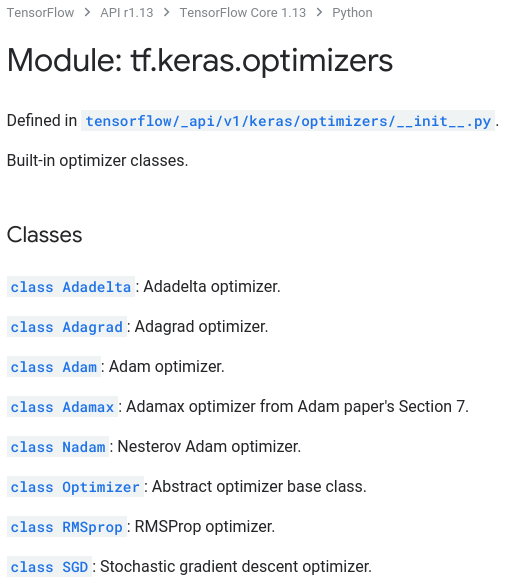
\includegraphics[scale=0.3]{tf-keras-optimizers.png}
 \\
        \end{tabular}
        \label{tab:tf-motivation}
    \end{table}
    
\end{frame}

\begin{frame}
    \frametitle{Motivation}
    \framesubtitle{PyTorch}
    
    \begin{table}
        \centering
        \begin{tabular}{c c}
        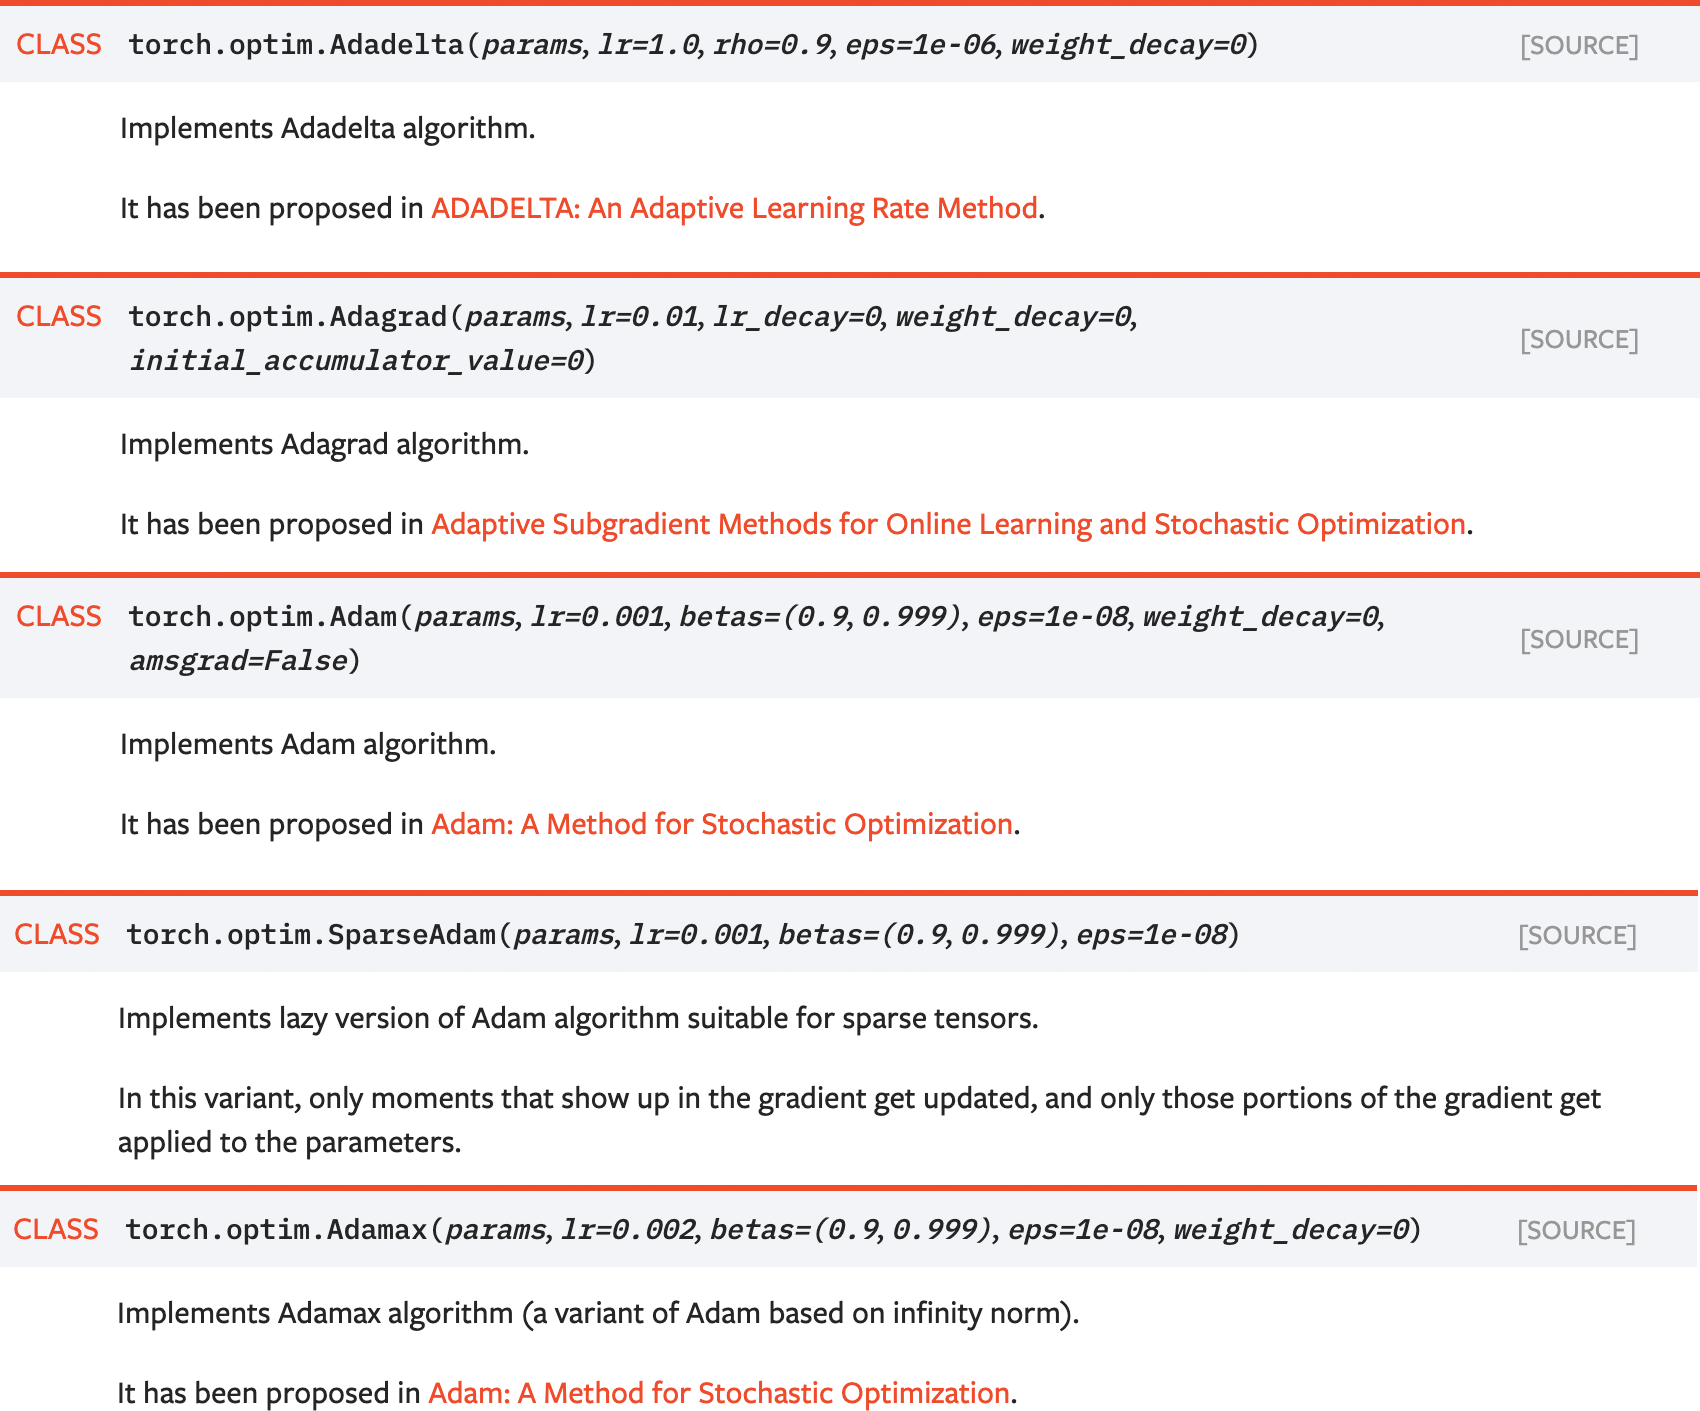
\includegraphics[width=0.5\columnwidth]{pytorch-algs-1.png} & 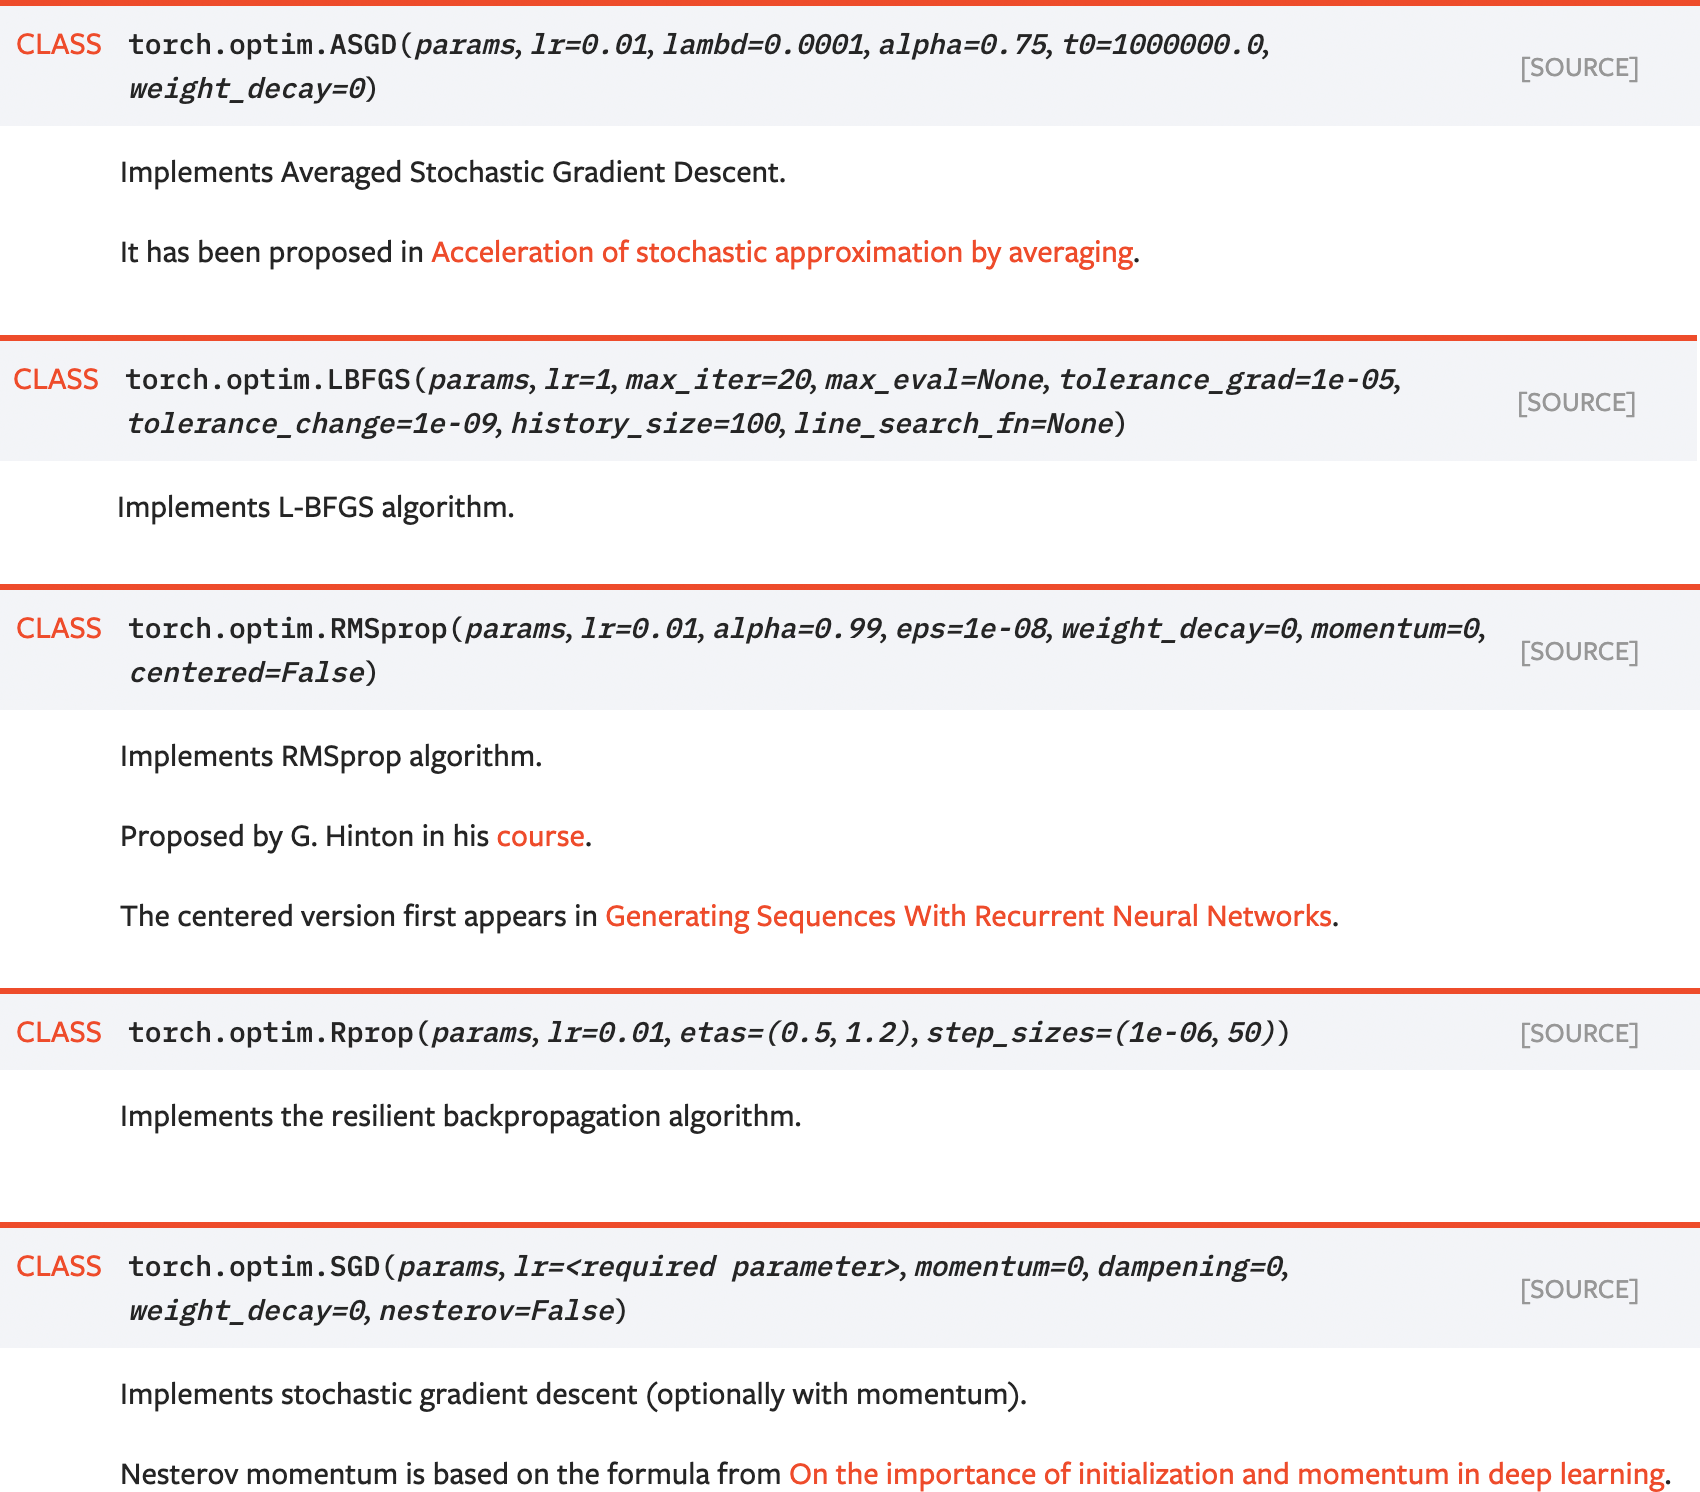
\includegraphics[width=0.5\columnwidth]{pytorch-algs-2.png} 
 \\
        \end{tabular}
        \label{tab:pytorch-motivation}
    \end{table}
    
\end{frame}

\begin{frame}
    \frametitle{Motivation}
    \framesubtitle{Caffe}
    
    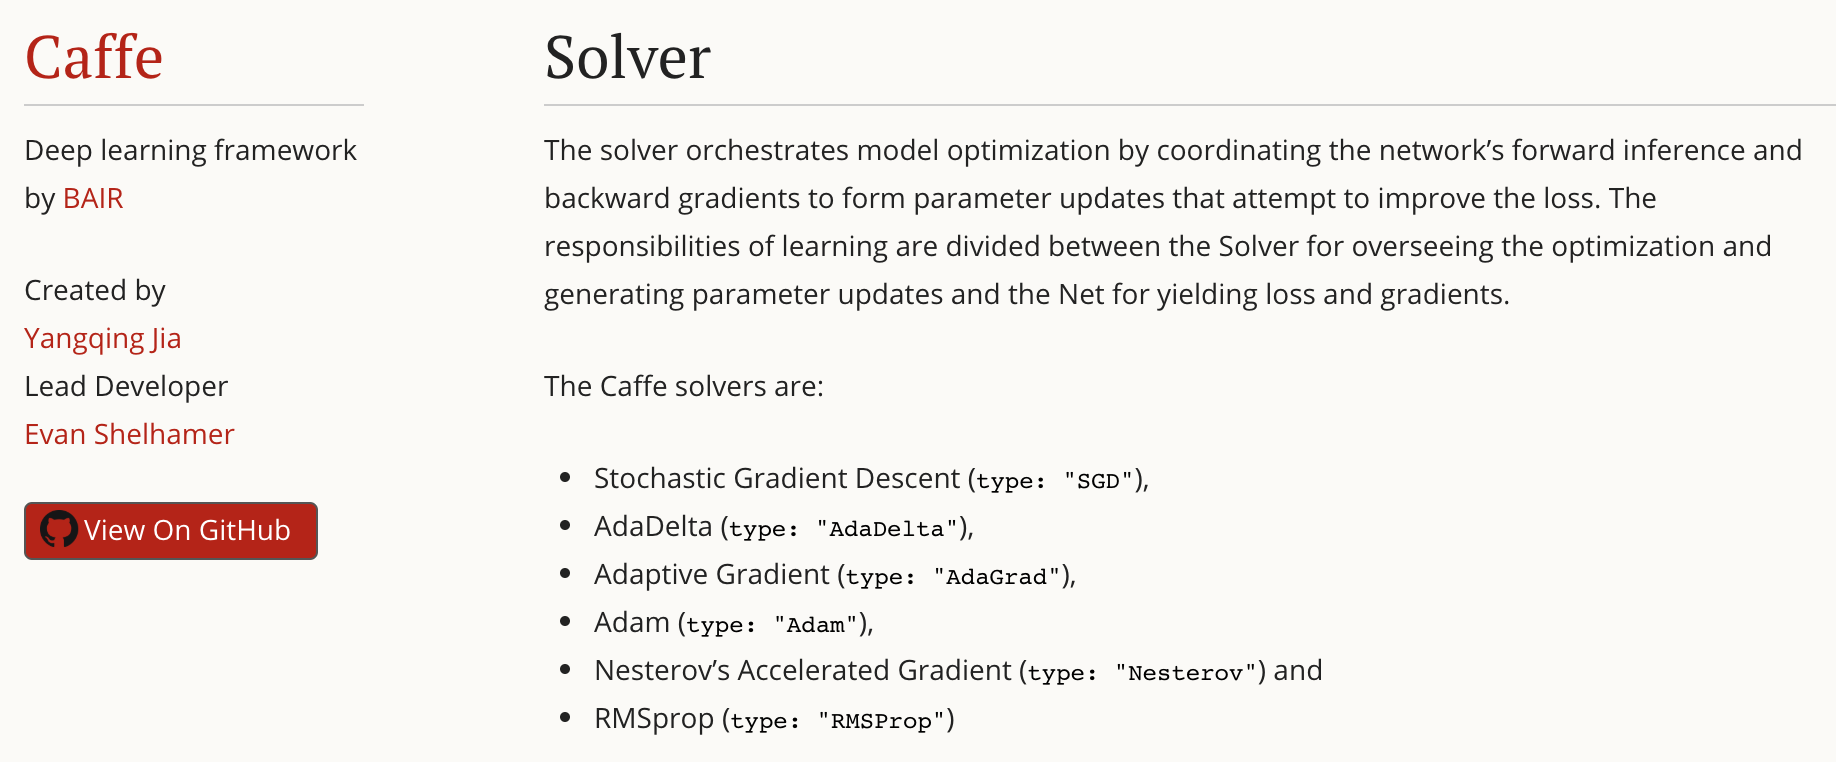
\includegraphics[width=1\columnwidth]{caffe-algs.png}
    
\end{frame}

\begin{frame}
    \frametitle{Motivation}
    \framesubtitle{Microsoft Cognitive Toolkit}
    
    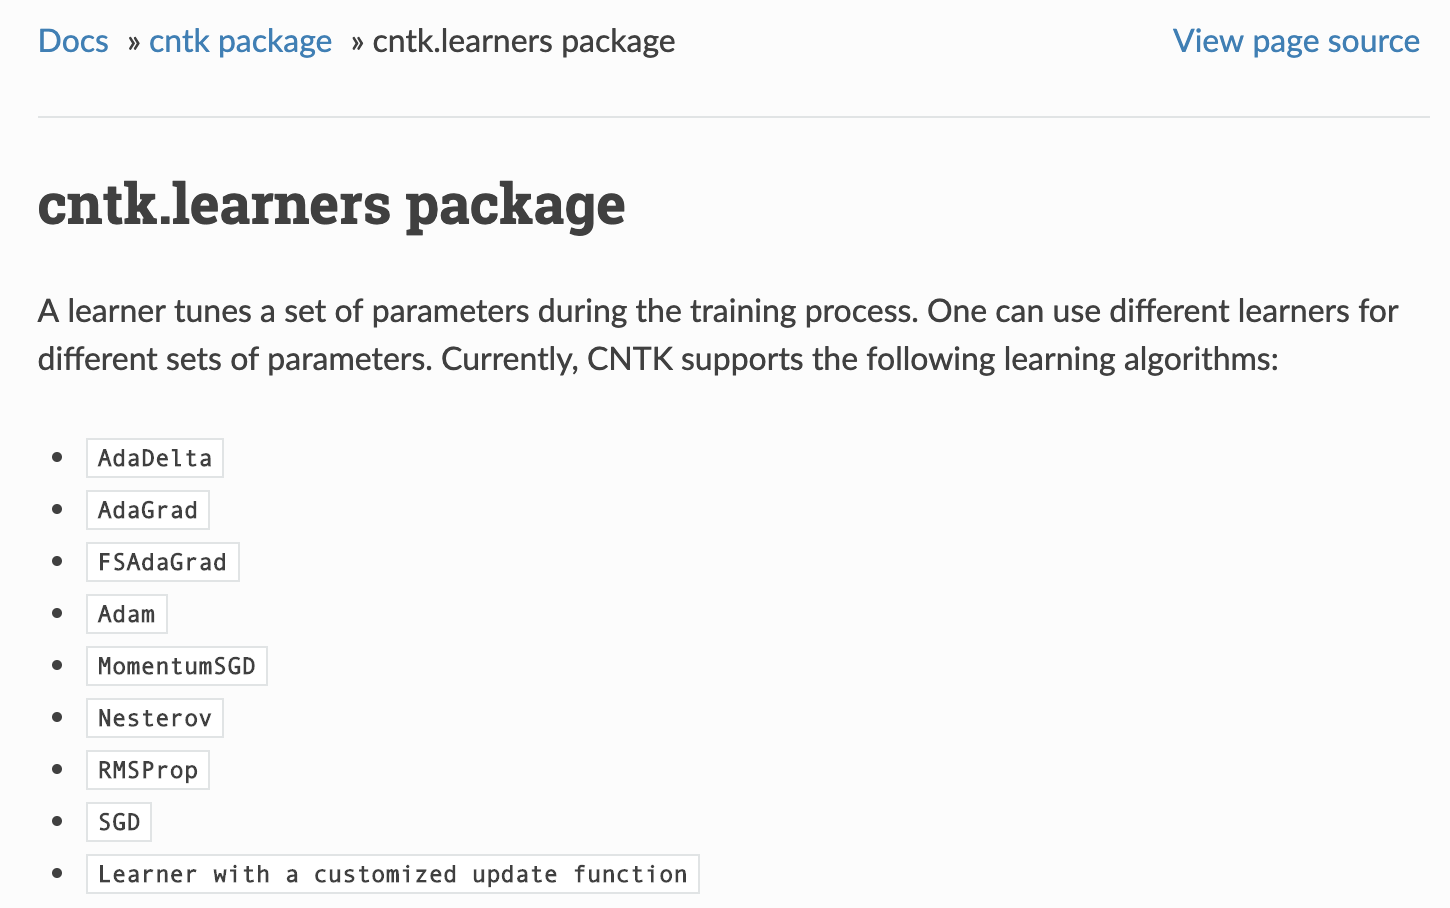
\includegraphics[width=1\columnwidth]{cntk-algs.png}
    
\end{frame}

\begin{frame}
    \frametitle{Gradient Descent Variants}
    
    \begin{tikzpicture}[
        decoration={shape backgrounds,shape size=1.5cm,shape=signal},
        signal from=west, signal to=east,
        paint/.style={decorate, draw=#1!50!black, fill=#1!50}]
        % \draw [help lines] grid (3,2);
        
        % \draw [paint=red, decoration={shape sep=.5cm}]
        % (0,2) -- (5,2);
        
        % \draw [paint=green, decoration={shape sep={1cm, between centers}}]
        % (0,1) -- (3,1);
        \draw [paint=blue, decoration={shape sep={1cm, between borders}}]
        (0,0) -- (5,0);
    \end{tikzpicture}
    
    
    \begin{tikzpicture}
          \tikzset{
            % bound/.style={
            %   draw,
            %   minimum height=2cm,
            %   inner sep=1em,
            % },
            arrow/.style={
              draw,
              minimum height=1cm,
              inner sep=1.1em,
              shape=signal,
              signal from=west,
              signal to=east,
              signal pointer angle=110,
              draw=#1!00!white, fill=#1!10!purple,
            }
          }
        %   \node[bound] (a) {A};
          \begin{scope}[start chain=transition going right,node distance=-\pgflinewidth]
            \node[arrow,on chain] {\textbf{\textcolor{white}{Batch GD}}};
            \node[arrow,on chain] {\textbf{\textcolor{white}{Stochastic GD}}};
            \node[arrow,on chain] {\textbf{\textcolor{white}{Mini-batch GD}}};
          \end{scope}
        %   \node[bound,right=1cm of transition-end]{B};
    \end{tikzpicture}
    
    % Math font has been overridden (IDK why!?)
    % I have used \mathnormal for all eqs.
    \begin{enumerate}
        \item 
        \begin{tabular}{c c}
             Batch GD (vanilla GD) &  $\mathnormal{\theta = \theta - \alpha . \nabla_\theta {J}(\theta)}$
        \end{tabular}
            \begin{itemize}
                \color{magenta}
                \item Calculates gradient for the whole data set for each update.
                \item Relatively far slower than other variants.
                \item Not able to update the model \textit{online}.
            \end{itemize}
        \item 
        \begin{tabular}{c c}
            Stochastic GD (SGD) &  $\mathnormal{\theta = \theta - \alpha . \nabla_{\theta} J(\theta; x^{(i)}; y^{(i)}) }$
        \end{tabular}
            \begin{itemize}
                \color{magenta}
                \item Frequent updates (one update at a time).
                \item Higher model variance.
                \item Potential better local minima (compared to vanilla GD).
            \end{itemize}
        \item 
        \begin{tabular}{c c}
            Mini-batch GD &  $\mathnormal{\theta = \theta - \alpha . \nabla_{\theta} J(\theta; x^{(i:i+m)}; y^{(i:i+m)})}$
        \end{tabular}
            \begin{itemize}
                \color{magenta}
                \item Reduction in variance (compared to SGD).
                \item More often batch sizes of 50-256.
            \end{itemize}
    \end{enumerate}

\end{frame}



% \begin{frame}{Plot of story}

%          \begin{tikzpicture}
%           \tikzset{
%             % bound/.style={
%             %   draw,
%             %   minimum height=2cm,
%             %   inner sep=1em,
%             % },
%             arrow/.style={
%               draw,
%               minimum height=1cm,
%               inner sep=1.1em,
%               shape=signal,
%               signal from=west,
%               signal to=east,
%               signal pointer angle=110,
%               draw=#1!00!white, fill=#1!10!green,
%             }
%           }
%           \begin{scope}[start chain=transition going right,node distance=-\pgflinewidth]
%             \node[arrow,on chain] {\textbf{\textcolor{white}{Momentum}}};
%             \node[arrow,on chain] {\textbf{\textcolor{white}{NAG}}};
%             \node[arrow,on chain] {\textbf{\textcolor{white}{AdaGrad}}};
%             \node[arrow,on chain] {\textbf{\textcolor{white}{AdaDelta}}};
%             \node[arrow,on chain] {\textbf{\textcolor{white}{RMSprop}}};
%             \node[arrow,on chain] {\textbf{\textcolor{white}{Adam}}};
%             \node[arrow,on chain] {\textbf{\textcolor{white}{NAdam}}};

%           \end{scope}
%     \end{tikzpicture}
% \end{frame}




\begin{frame}
    \frametitle{Momentum}
    
    % \begin{tikzpicture}
    %       \tikzset{
    %         % bound/.style={
    %         %   draw,
    %         %   minimum height=2cm,
    %         %   inner sep=1em,
    %         % },
    %         arrow/.style={
    %           draw,
    %           minimum height=1cm,
    %           inner sep=1.1em,
    %           shape=signal,
    %           signal from=west,
    %           signal to=east,
    %           signal pointer angle=110,
    %           draw=#1!00!white, fill=#1!10!green,
    %         }
    %       }
    %       \begin{scope}[start chain=transition going right,node distance=-\pgflinewidth]
    %         \node[arrow,on chain] {\textbf{\textcolor{white}{Momentum}}};
    %       \end{scope}
    % \end{tikzpicture}
    
    The momentum term increases for dimensions whose gradients point in the same directions and reduces updates for dimensions whose gradients change directions. 
    
    \begin{equation}
        \begin{aligned} v_{t} &=\gamma v_{t-1}+\eta \nabla_{\theta} J(\theta) \\ \theta &=\theta-v_{t} \end{aligned}
    \end{equation}
    
    As a result, we gain faster convergence and reduced oscillation.
    
\end{frame}

\begin{frame}
    \frametitle{Nesterov Accelerated Gradient}
    
    % \begin{tikzpicture}
    %       \tikzset{
    %         % bound/.style={
    %         %   draw,
    %         %   minimum height=2cm,
    %         %   inner sep=1em,
    %         % },
    %         arrow/.style={
    %           draw,
    %           minimum height=1cm,
    %           inner sep=1.1em,
    %           shape=signal,
    %           signal from=west,
    %           signal to=east,
    %           signal pointer angle=110,
    %           draw=#1!00!white, fill=#1!10!green,
    %         }
    %       }
    %       \begin{scope}[start chain=transition going right,node distance=-\pgflinewidth]
    %         \node[arrow,on chain] {\textbf{\textcolor{white}{Momentum}}};
    %         \node[arrow,on chain] {\textbf{\textcolor{white}{NAG}}};

    %       \end{scope}
    % \end{tikzpicture}
    
    Computing $\theta-\gamma v_{t-1}$ thus gives us an approximation of \textbf{the next position of the parameters} a rough idea where our parameters are going to be. 
    \begin{equation}
         \begin{aligned} v_{t} &=\gamma v_{t-1}+\eta \nabla_{\theta} J\left(\theta-\gamma v_{t-1}\right) \\ \theta &=\theta-v_{t} \end{aligned}
    \end{equation}
\end{frame}

\begin{frame}
    \frametitle{AdaGrad}
    
    % \begin{tikzpicture}
    %       \tikzset{
    %         % bound/.style={
    %         %   draw,
    %         %   minimum height=2cm,
    %         %   inner sep=1em,
    %         % },
    %         arrow/.style={
    %           draw,
    %           minimum height=1cm,
    %           inner sep=1.1em,
    %           shape=signal,
    %           signal from=west,
    %           signal to=east,
    %           signal pointer angle=110,
    %           draw=#1!00!white, fill=#1!10!green,
    %         }
    %       }
    %       \begin{scope}[start chain=transition going right,node distance=-\pgflinewidth]
    %         \node[arrow,on chain] {\textbf{\textcolor{white}{Momentum}}};
    %         \node[arrow,on chain] {\textbf{\textcolor{white}{NAG}}};

    %       \end{scope}
    % \end{tikzpicture}
    
    Adapts the learning rate to the parameters:
    \begin{itemize}
        \item smaller updates (i.e. low learning rates) for parameters associated with frequently occurring features,
        \item larger updates (i.e. high learning rates) for parameters associated with infrequent features.
    \end{itemize}
    
    
    
    \begin{equation}
        g_{t, i}=\nabla_{\theta} J\left(\theta_{t, i}\right)
    \end{equation}
    
    \begin{equation}
\theta_{t+1, i}=\theta_{t, i}-\frac{\eta}{\sqrt{G_{t, i i}+\epsilon}} \cdot g_{t, i}
\end{equation}

$G_{t} \in \mathbb{R}^{d \times d}$ is a diagonal matrix where each diagonal element $i,i$ is the sum of the squares of the gradients respect to $\theta_i$ up to time step $t$.

\end{frame}

\begin{frame}
    \frametitle{AdaDelta}
    Derived from AdaGrad but to enhance it's monotonically decreasing learning rate.
    
    \begin{equation}
E\left[g^{2}\right]_{t}=\gamma E\left[g^{2}\right]_{t-1}+(1-\gamma) g_{t}^{2}
\end{equation}

\begin{equation}
\Delta \theta_{t}=-\frac{\eta}{\sqrt{E\left[g^{2}\right]_{t}+\epsilon}} g_{t}
\end{equation}

\begin{equation}
E\left[\Delta \theta^{2}\right]_{t}=\gamma E\left[\Delta \theta^{2}\right]_{t-1}+(1-\gamma) \Delta \theta_{t}^{2}
\end{equation}

\begin{equation}
\begin{aligned} \Delta \theta_{t} &=-\frac{R M S[\Delta \theta]_{t-1}}{R M S[g]_{t}} g_{t} \\ \theta_{t+1} &=\theta_{t}+\Delta \theta_{t} \end{aligned}
\end{equation}
    
\end{frame}


\begin{frame}
    \frametitle{RMSprop}
    
    % \begin{tikzpicture}
    %       \tikzset{
    %         % bound/.style={
    %         %   draw,
    %         %   minimum height=2cm,
    %         %   inner sep=1em,
    %         % },
    %         arrow/.style={
    %           draw,
    %           minimum height=1cm,
    %           inner sep=1.1em,
    %           shape=signal,
    %           signal from=west,
    %           signal to=east,
    %           signal pointer angle=110,
    %           draw=#1!00!white, fill=#1!10!green,
    %         }
    %       }
    %       \begin{scope}[start chain=transition going right,node distance=-\pgflinewidth]
    %         \node[arrow,on chain] {\textbf{\textcolor{white}{Momentum}}};
    %         \node[arrow,on chain] {\textbf{\textcolor{white}{NAG}}};

    %       \end{scope}
    % \end{tikzpicture}
    
    Same time with AdaDelta to address the intense decrease in learning rate of AdaGrad. 
    
    \begin{equation}
\begin{aligned} E\left[g^{2}\right]_{t} &=0.9 E\left[g^{2}\right]_{t-1}+0.1 g_{t}^{2} \\ \theta_{t+1} &=\theta_{t}-\frac{\eta}{\sqrt{E\left[g^{2}\right]_{t}+\epsilon}} g_{t} \end{aligned}
\end{equation}
    
\end{frame}



\begin{frame}
    \frametitle{Adam}
    
    % \begin{tikzpicture}
    %       \tikzset{
    %         % bound/.style={
    %         %   draw,
    %         %   minimum height=2cm,
    %         %   inner sep=1em,
    %         % },
    %         arrow/.style={
    %           draw,
    %           minimum height=1cm,
    %           inner sep=1.1em,
    %           shape=signal,
    %           signal from=west,
    %           signal to=east,
    %           signal pointer angle=110,
    %           draw=#1!00!white, fill=#1!10!green,
    %         }
    %       }
    %       \begin{scope}[start chain=transition going right,node distance=-\pgflinewidth]
    %         \node[arrow,on chain] {\textbf{\textcolor{white}{Momentum}}};
    %         \node[arrow,on chain] {\textbf{\textcolor{white}{NAG}}};

    %       \end{scope}
    % \end{tikzpicture}
    
    Keeps the track of decaying average of past:
    \begin{itemize}
        \item squared gradient similar to AdaDelta and RMSprop, and
        \item gradient similar to momentum.
    \end{itemize}
    
    \begin{equation}
\begin{aligned} m_{t} &=\beta_{1} m_{t-1}+\left(1-\beta_{1}\right) g_{t} \\ v_{t} &=\beta_{2} v_{t-1}+\left(1-\beta_{2}\right) g_{t}^{2} \end{aligned}
\end{equation}

\begin{equation}
\theta_{t+1}=\theta_{t}-\frac{\eta}{\sqrt{v_{t}}+\epsilon} m_{t}
\end{equation}
    
\end{frame}


\begin{frame}
    \frametitle{NAdam}
    
    From momentum:
    \begin{equation}
        \begin{aligned} v _ { t } & = \gamma v _ { t - 1 } + \eta \nabla _ { \theta } J ( \theta ) \\ \theta & = \theta - v _ { t } \end{aligned}
    \end{equation}
    
    Rewrite it now:
    \begin{equation}
        \begin{aligned} g _ { t } & = \nabla _ { \theta _ { t } } J \left( \theta _ { t } \right) \\ m _ { t } & = \gamma m _ { t - 1 } + \eta g _ { t } \\ \theta _ { t + 1 } & = \theta _ { t } - m _ { t } \end{aligned}
    \end{equation}
    
    \begin{equation}
        \begin{aligned} g _ { t } & = \nabla _ { \theta _ { t } } J \left( \theta _ { t } \right) \\ m _ { t } & = \gamma m _ { t - 1 } + \eta g _ { t } \\ \theta _ { t + 1 } & = \theta _ { t } - \left( \gamma m _ { t } + \eta g _ { t } \right) \end{aligned}
    \end{equation}
    
   

\end{frame}

\begin{frame}

 \begin{equation}
        \begin{aligned} m _ { t } & = \beta _ { 1 } m _ { t - 1 } + \left( 1 - \beta _ { 1 } \right) g _ { t } \\ \hat { m } _ { t } & = \frac { m _ { t } } { 1 - \beta _ { 1 } ^ { t } } \\ \theta _ { t + 1 } & = \theta _ { t } - \frac { \eta } { \sqrt { \hat { v } _ { t } } + \epsilon } \hat { m } _ { t } \end{aligned}
    \end{equation}
    
    \begin{equation}
        \theta _ { t + 1 } = \theta _ { t } - \frac { \eta } { \sqrt { \hat { v } _ { t } } + \epsilon } \left( \beta _ { 1 } \hat { m } _ { t } + \frac { \left( 1 - \beta _ { 1 } \right) g _ { t } } { 1 - \beta _ { 1 } ^ { t } } \right)
    \end{equation}
\end{frame}

\begin{fram}
    \frametitle{Show Time!}
    
    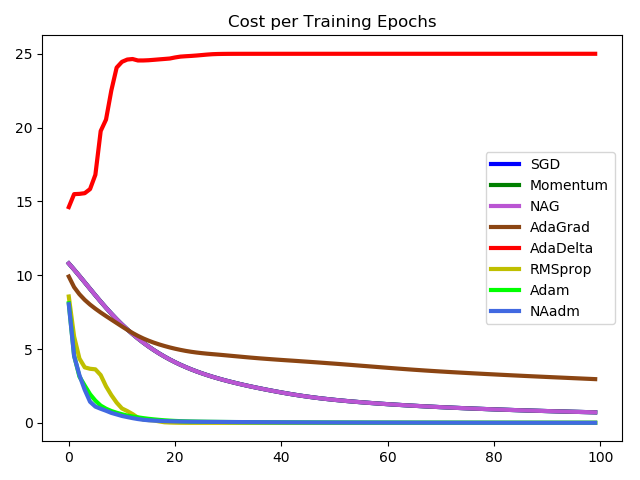
\includegraphics[scale=0.5]{presentation/MathOpt-proj/myplot.png}
\end{fram}

\begin{frame}
    \center \textbf{Questions?}
\end{frame}

\end{document}
